\documentclass[11pt]{article}

% ---------- Packages ----------
\usepackage[utf8]{inputenc}
\usepackage[T1]{fontenc}
\usepackage{amsmath, amssymb, amsthm}
\usepackage{geometry}
\usepackage{booktabs}
\usepackage{array}
\usepackage{multirow}
\usepackage{xcolor}
\usepackage{enumitem}
\usepackage{hyperref}
\usepackage{graphicx}
\usepackage{float}
\usepackage{listings}
\usepackage{tikz}
\usetikzlibrary{arrows.meta, positioning, shapes.geometric, calc}

\geometry{a4paper, margin=1in}
\hypersetup{
    colorlinks=true,
    linkcolor=blue!60!black,
    urlcolor=blue!60!black,
    citecolor=blue!60!black
}

% ---------- Custom commands ----------
\newcommand{\OL}{\mathit{OL}}
\newcommand{\OW}{\mathit{OW}}
\newcommand{\OH}{\mathit{OH}}
\newcommand{\WB}{\mathit{WB}}
\newcommand{\TW}{\mathit{TW}}
\newcommand{\FH}{\mathit{FH}}
\newcommand{\RH}{\mathit{RH}}
\newcommand{\given}{\,\vert\,}
\newcommand{\Norm}{\mathcal{N}}
\newcommand{\bmu}{\boldsymbol{\mu}}
\newcommand{\bSigma}{\boldsymbol{\Sigma}}
\newcommand{\bx}{\mathbf{x}}
\newcommand{\bz}{\mathbf{z}}
\newcommand{\bX}{\mathbf{X}}
\newcommand{\Lmat}{\mathbf{L}}
\newcommand{\Imat}{\mathbf{I}}
\newcommand{\T}{^{\!\top}}

\theoremstyle{definition}
\newtheorem{remark}{Remark}

% ---------- Listings style ----------
\definecolor{codebg}{gray}{0.96}
\definecolor{codekw}{rgb}{0.10,0.10,0.55}
\definecolor{codecm}{rgb}{0.30,0.50,0.30}
\lstset{
    basicstyle=\ttfamily\footnotesize,
    backgroundcolor=\color{codebg},
    keywordstyle=\color{codekw}\bfseries,
    commentstyle=\color{codecm}\itshape,
    stringstyle=\color{purple!60!black},
    language=Python,
    breaklines=true,
    frame=single,
    framesep=4pt,
    showstringspaces=false,
    columns=fullflexible,
    keepspaces=true,
}

\title{\textbf{Fair Sampling from Per-Type Joint Gaussian Vehicle Models}\\[4pt]
\large The Generative Demo: From the Cars Database to a Rendered Draw}
\author{Project Report}
\date{\today}

\begin{document}
\maketitle

\begin{abstract}
\noindent This report documents the \emph{fair-sampling} (generative) branch of the vehicle pipeline, implemented in \texttt{rendering/fairsample\_rendering.py} on top of the parametric polygon model in \texttt{rendering/car\_models\_core\_new.py}. Unlike \emph{reconstruction}, which takes a real detected car and recovers the most likely interior proportions by conditioning on four measured exterior dimensions, fair sampling takes \emph{no} car as input. Given only a category name (sedan, SUV, truck, or van) it fits an $11$-dimensional joint Gaussian to every real vehicle of that type in the cars database, draws unbiased samples from that distribution, and renders each draw side by side so that the natural diversity of the category becomes visible at a glance. We give the full pipeline, the exact data cleaning and variable mapping, the maximum-likelihood estimation of the mean $\bmu$ and covariance $\bSigma$, the Cholesky-based sampling identity $\bx=\bmu+\Lmat\bz$ with a proof that it reproduces $\Norm(\bmu,\bSigma)$ exactly, and the mapping from a sampled dimension vector to renderable geometry. We close by contrasting the two probabilistic operations the project relies on --- the deterministic conditional mean used for reconstruction and the stochastic fair draw used here.
\end{abstract}

\tableofcontents
\vspace{1em}
\hrule
\vspace{1em}

% =====================================================================
\section{Motivation: Why Sample at All?}
% =====================================================================

The project uses one statistical object --- a multivariate Gaussian over vehicle dimensions --- in two very different ways.

\begin{description}[leftmargin=1.5em, style=nextline]
  \item[Reconstruction (deterministic).] A real car is detected; an upstream stage measures its four exterior dimensions $b=(\OW,\WB,\OH,\OL)$. We want the single most plausible set of interior proportions $a=(A,C,D,E,\FH,\RH,\TW)$ consistent with those measurements. The answer is the \emph{conditional mean} $\mathbb{E}[a\given b]$, a closed-form, repeatable vector. The same car always reconstructs to the same shape.
  \item[Fair sampling (stochastic).] No car is given. We ask: ``\emph{What does the population of real sedans actually look like, in all its variety?}'' The answer is a set of \emph{independent draws} from the full joint distribution of all $11$ dimensions. Each draw is a different, plausible vehicle; together they portray the spread of the category.
\end{description}

\noindent The professor's request --- ``sample fairly from a joint Gaussian distribution to show the diversity in each category'' --- is the second operation. ``Fair'' is the key word: every draw must appear with frequency \emph{proportional to its true probability density}, so that common body shapes show up often and unusual ones rarely, with no artificial bias toward the average. This report explains exactly how that is achieved.

% =====================================================================
\section{Pipeline Overview}
% =====================================================================

\begin{figure}[H]
\centering
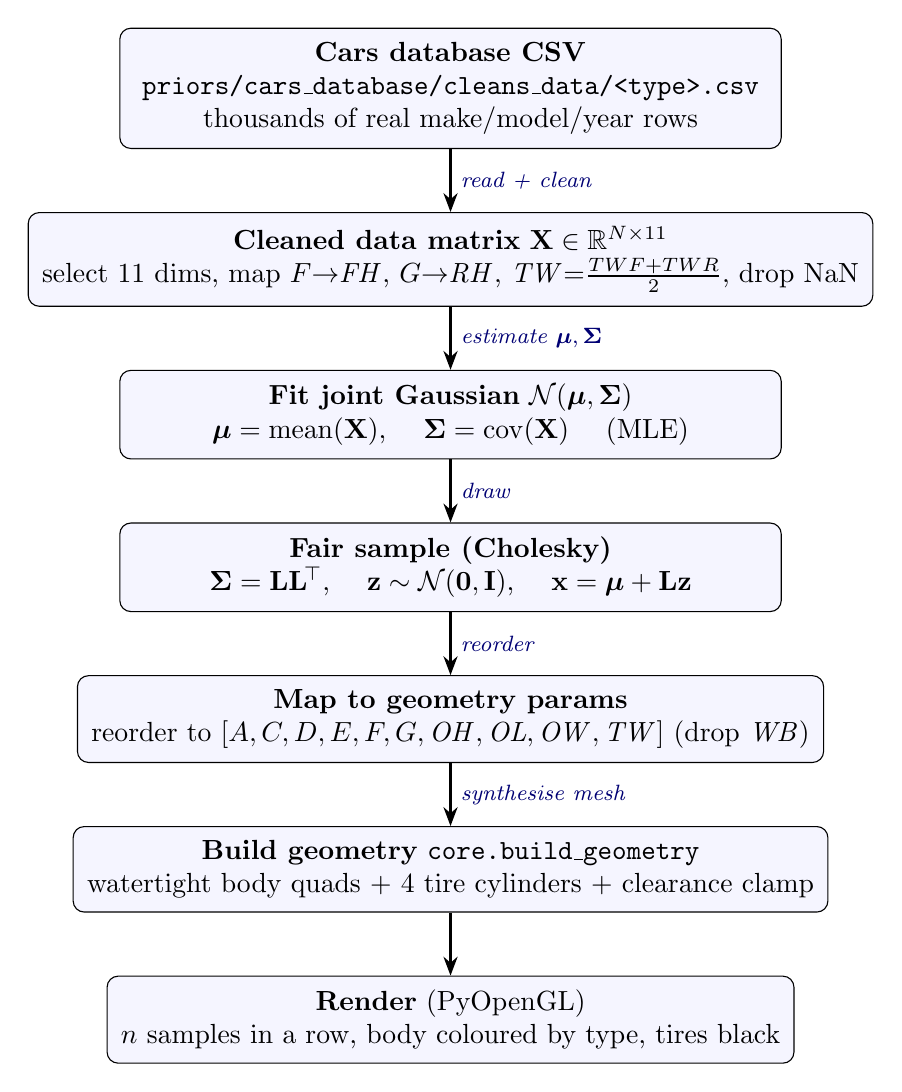
\begin{tikzpicture}[
    node distance=8mm,
    box/.style={draw, rounded corners, align=center, inner sep=5pt, minimum width=8.4cm, fill=blue!4},
    lbl/.style={font=\footnotesize\itshape, align=center, text=blue!45!black},
    arr/.style={-{Stealth[length=2.4mm]}, thick}
]
\node[box] (csv)  {\textbf{Cars database CSV}\\ \texttt{priors/cars\_database/cleans\_data/<type>.csv}\\ thousands of real make/model/year rows};
\node[box, below=of csv] (mat) {\textbf{Cleaned data matrix} $\bX\in\mathbb{R}^{N\times 11}$\\ select 11 dims, map $F{\to}\FH$, $G{\to}\RH$, $\TW{=}\tfrac{TWF+TWR}{2}$, drop NaN};
\node[box, below=of mat] (gauss) {\textbf{Fit joint Gaussian} $\Norm(\bmu,\bSigma)$\\ $\bmu=\mathrm{mean}(\bX)$, \quad $\bSigma=\mathrm{cov}(\bX)$ \quad (MLE)};
\node[box, below=of gauss] (samp) {\textbf{Fair sample (Cholesky)}\\ $\bSigma=\Lmat\Lmat\T$, \quad $\bz\sim\Norm(\mathbf{0},\Imat)$, \quad $\bx=\bmu+\Lmat\bz$};
\node[box, below=of samp] (param) {\textbf{Map to geometry params}\\ reorder to $[A,C,D,E,F,G,\OH,\OL,\OW,\TW]$ (drop $\WB$)};
\node[box, below=of param] (geom) {\textbf{Build geometry} \texttt{core.build\_geometry}\\ watertight body quads $+$ 4 tire cylinders $+$ clearance clamp};
\node[box, below=of geom] (render) {\textbf{Render} (PyOpenGL)\\ $n$ samples in a row, body coloured by type, tires black};

\draw[arr] (csv)   -- (mat)   node[lbl, midway, right] {read + clean};
\draw[arr] (mat)   -- (gauss) node[lbl, midway, right] {estimate $\bmu,\bSigma$};
\draw[arr] (gauss) -- (samp)  node[lbl, midway, right] {draw};
\draw[arr] (samp)  -- (param) node[lbl, midway, right] {reorder};
\draw[arr] (param) -- (geom)  node[lbl, midway, right] {synthesise mesh};
\draw[arr] (geom)  -- (render);
\end{tikzpicture}
\caption{The fair-sampling pipeline. Everything left of rendering is pure NumPy/pandas; only the last stage touches OpenGL.}
\label{fig:pipeline}
\end{figure}

% =====================================================================
\section{Stage 1 --- From the Database to a Data Matrix}
% =====================================================================

Each category has its own cleaned CSV, e.g. \texttt{sedan.csv} ($\approx 5{,}197$ rows), where every row is one real make/model/year with its measured dimensions in centimetres. The function \texttt{build\_joint\_gaussian} reads the file and prepares the modelling variables.

\paragraph{The 11 joint variables.} We model the joint distribution of
\begin{equation}
\text{\texttt{JOINT\_VARS}} \;=\; \big[\underbrace{A,\;C,\;D,\;E,\;\FH,\;\RH,\;\TW}_{\text{7 interior / proportion}},\;\;\underbrace{\OW,\;\WB,\;\OH,\;\OL}_{\text{4 exterior}}\big].
\end{equation}
These are exactly the $a$ and $b$ groups of the reconstruction model, now treated as one undivided $11$-vector because fair sampling lets \emph{all} of them vary together.

\begin{table}[H]
\centering
\begin{tabular}{cl}
\toprule
\textbf{Symbol} & \textbf{Meaning} \\
\midrule
$\OL,\OW,\OH$ & overall length, width, height \\
$\WB$         & wheelbase (sampled, but not placed geometrically) \\
$A$           & front bumper to base of windshield (hood/nose run) \\
$C$           & side-window (greenhouse) height \\
$D$           & door height below the window \\
$E$           & greenhouse width / roof inset \\
$\FH,\RH$     & front and rear axle offsets (CSV columns $F$, $G$) \\
$\TW$         & mean track width, $\tfrac{1}{2}(TWF+TWR)$ \\
\bottomrule
\end{tabular}
\caption{The 11 modelled dimensions.}
\end{table}

\paragraph{Cleaning and variable mapping.} Three normalisations align the raw CSV with the convention used by the reconstruction models (\texttt{eval/get\_multivariate\_model\_and\_make\_model.py}):
\begin{enumerate}[leftmargin=2em]
  \item \textbf{Header whitespace} is stripped (\texttt{'OH '} $\to$ \texttt{'OH'}, \texttt{'TWR '} $\to$ \texttt{'TWR'}).
  \item \textbf{Renaming:} the CSV's $F$ and $G$ become $\FH$ and $\RH$.
  \item \textbf{Track width} is derived: $\TW=\tfrac{1}{2}(TWF+TWR)$.
\end{enumerate}
The 11 columns are then coerced to numeric and any row with a missing value is dropped, leaving $N$ complete rows (e.g. $\approx 4{,}354$ usable sedans). The result is the data matrix
\begin{equation}
\bX=\begin{bmatrix} \bx_1\T \\ \vdots \\ \bx_N\T \end{bmatrix}\in\mathbb{R}^{N\times 11},
\qquad \bx_i\in\mathbb{R}^{11}.
\end{equation}

\begin{lstlisting}[caption={Data preparation (\texttt{build\_joint\_gaussian}).}]
df = pd.read_csv(csv)
df.columns = df.columns.str.strip()          # 'OH ' -> 'OH'
df = df.rename(columns={'F': 'FH', 'G': 'RH'})
df['TW'] = (pd.to_numeric(df['TWF']) + pd.to_numeric(df['TWR'])) / 2.0
sdf = df[JOINT_VARS].apply(pd.to_numeric, errors='coerce').dropna()
mu    = sdf.mean().values                     # 11-vector
sigma = np.cov(sdf.values, rowvar=False)      # 11 x 11
\end{lstlisting}

% =====================================================================
\section{Stage 2 --- Fitting the Joint Gaussian}
% =====================================================================

We model the 11 dimensions as jointly Gaussian, $\bx\sim\Norm(\bmu,\bSigma)$, and fit the two parameters by their maximum-likelihood estimators --- the sample mean and sample covariance.

\paragraph{Mean.} The per-variable average, $\bmu\in\mathbb{R}^{11}$:
\begin{equation}
\mu_j=\frac{1}{N}\sum_{i=1}^{N}X_{ij}, \qquad j=1,\dots,11.
\end{equation}

\paragraph{Covariance.} The $11\times11$ matrix (\texttt{np.cov(..., rowvar=False)} uses the unbiased $N{-}1$ normaliser):
\begin{equation}
\Sigma_{jk}=\frac{1}{N-1}\sum_{i=1}^{N}\big(X_{ij}-\mu_j\big)\big(X_{ik}-\mu_k\big).
\end{equation}

\noindent The structure of $\bSigma$ is what makes the samples physically coherent:
\begin{itemize}[leftmargin=2em]
  \item the \textbf{diagonal} $\Sigma_{jj}=\mathrm{Var}(\text{dim}_j)$ measures how much each dimension spreads (length varies a lot across sedans; track width far less);
  \item the \textbf{off-diagonals} $\Sigma_{jk}$ encode \emph{co-variation} --- a long car tends to have a long wheelbase and a taller body. These correlations are precisely what keep a sampled vehicle from being an incoherent mix of a small car's roof on a limousine's chassis.
\end{itemize}

\begin{remark}
$(\bmu,\bSigma)$ are the maximum-likelihood estimates of a multivariate Gaussian given i.i.d.\ data. A consistency check from earlier work: the $\bmu$ computed here from \texttt{sedan.csv} matches the stored reconstruction model means in \texttt{priors/models/gaussian\_model\_sedan\_*.npz} (e.g.\ $A{=}130.8$, $\OW{=}184.7$, $\OL{=}473.1$), confirming both code paths read the same data the same way.
\end{remark}

% =====================================================================
\section{Stage 3 --- Fair Sampling via the Cholesky Factor}
% =====================================================================

A \textbf{fair} sample is an honest i.i.d.\ draw from the fitted distribution: each candidate vehicle $\bx$ is produced with frequency equal to its density
\begin{equation}
p(\bx)=\frac{1}{(2\pi)^{11/2}\,|\bSigma|^{1/2}}
        \exp\!\Big(-\tfrac12(\bx-\bmu)\T\bSigma^{-1}(\bx-\bmu)\Big).
\label{eq:density}
\end{equation}
We never evaluate \eqref{eq:density} directly. Instead we exploit the fact that an affine map of a standard normal is Gaussian, and choose the map so its mean and covariance equal $\bmu$ and $\bSigma$.

\paragraph{The three-step recipe.}
\begin{align}
\textbf{(1) Factor: }   \quad & \bSigma=\Lmat\Lmat\T, \qquad \Lmat \text{ lower-triangular (Cholesky).}\\
\textbf{(2) Draw: }     \quad & \bz\sim\Norm(\mathbf{0},\Imat_{11}), \qquad 11 \text{ independent unit normals.}\\
\textbf{(3) Transform: }\quad & \boxed{\;\bx=\bmu+\Lmat\bz\;}
\end{align}
In code a tiny jitter $\varepsilon\Imat$ ($\varepsilon=10^{-6}$) is added before factoring to guarantee numerical positive-definiteness:

\begin{lstlisting}[caption={Fair draw (\texttt{fair\_samples}).}]
L = np.linalg.cholesky(sigma + 1e-6 * np.eye(len(mu)))
x = mu + L @ rng.standard_normal(len(mu))
# redraw only if a physical size came out non-positive (impossible, not unlikely)
if x[OW] > 0 and x[OH] > 0 and x[OL] > 0:
    accept(x)
\end{lstlisting}

\subsection{Proof that \texorpdfstring{$\bx=\bmu+\Lmat\bz$}{x = mu + L z} reproduces \texorpdfstring{$\Norm(\bmu,\bSigma)$}{N(mu,Sigma)} exactly}

A linear transformation of a Gaussian vector is Gaussian, so $\bx$ is Gaussian and is determined entirely by its first two moments.

\paragraph{Mean.} Using linearity of expectation and $\mathbb{E}[\bz]=\mathbf{0}$,
\begin{equation}
\mathbb{E}[\bx]=\mathbb{E}[\bmu+\Lmat\bz]=\bmu+\Lmat\,\mathbb{E}[\bz]=\bmu+\Lmat\cdot\mathbf{0}=\bmu.
\end{equation}

\paragraph{Covariance.} Using $\mathrm{Cov}(\bz)=\Imat$ and the identity $\mathrm{Cov}(\mathbf{A}\bz)=\mathbf{A}\,\mathrm{Cov}(\bz)\,\mathbf{A}\T$ (a constant shift $\bmu$ does not affect covariance),
\begin{equation}
\mathrm{Cov}(\bx)=\mathrm{Cov}(\Lmat\bz)=\Lmat\,\mathrm{Cov}(\bz)\,\Lmat\T=\Lmat\,\Imat\,\Lmat\T=\Lmat\Lmat\T=\bSigma.
\end{equation}

\noindent Therefore $\bx\sim\Norm(\bmu,\bSigma)$ --- identical to the fitted distribution. \hfill$\blacksquare$

\subsection{What the factor \texorpdfstring{$\Lmat$}{L} does, geometrically}

The vector $\bz$ is an isotropic ``unit blob'' of probability: independent components, unit variance in every direction. Multiplying by $\Lmat$ stretches and shears that blob into the elongated, tilted ellipsoid of real vehicles. The stretch along each correlated direction is exactly what makes a sampled long car \emph{also} receive a long wheelbase and a taller body. Because an affine map with $|\det\Lmat|\neq0$ preserves relative densities, the procedure is \emph{fair}: common shapes (near the centre of the ellipsoid) are drawn often, extreme shapes (in the tails) rarely. No dimension is fixed and nothing is conditioned --- this is \emph{full-joint} sampling, in which all 11 variables vary simultaneously.

\begin{remark}[The only intervention]
The accept/redraw guard rejects a draw only if $\OW$, $\OH$, or $\OL$ comes out non-positive --- a physically \emph{impossible} vehicle, not merely an unlikely one. With realistic means many standard deviations above zero this almost never fires, so it does not measurably distort the distribution.
\end{remark}

% =====================================================================
\section{Stage 4 --- Mapping a Sample to Geometry Parameters}
% =====================================================================

The mesh builder \texttt{build\_geometry} expects a 10-vector in the order \texttt{PARAM\_NAMES} $=[A,C,D,E,F,G,\OH,\OL,\OW,\TW]$. The helper \texttt{to\_geometry\_params} reorders the sampled 11-vector and drops one entry:
\begin{equation}
\underbrace{[A,C,D,E,\FH,\RH,\TW,\OW,\WB,\OH,\OL]}_{\text{sampled } \bx,\ \text{11 dims}}
\;\longrightarrow\;
\underbrace{[A,C,D,E,\underbrace{\FH}_{F},\underbrace{\RH}_{G},\OH,\OL,\OW,\TW]}_{\text{geometry params, 10 dims}}.
\end{equation}
$\WB$ is sampled (so its correlations still shape every other dimension) and printed for inspection, but it is \emph{not} placed geometrically: in this parametric model the axle positions are set directly by the overhang offsets $F$ and $G$, so wheelbase only ever served to condition the prior.

% =====================================================================
\section{Stage 5 --- Building and Rendering the Vehicle}
% =====================================================================

For each accepted sample the renderer calls \texttt{core.build\_geometry(params, type)}, which turns the dimensions into a watertight body and four wheels.

\paragraph{Body and wheels.} The body is assembled as quads from the type's ``model car'' recipe (tapered nose of length $A$, beltline at $\OH-C$, body floor at $\OH-C-D$, greenhouse width $E$, and a type-specific roof from the \texttt{SHAPE} table). Four tire cylinders of type-specific radius (\texttt{tire\_r}: sedan $43.18$, SUV/van $46.0$, truck $55.0$\,cm) are placed at the front axle $z=-F$ and rear axle $z=-(\OL-G)$.

\paragraph{Ground-clearance clamp.} Because the body box is flat-bottomed (no wheel arches), the visible part of a grounded wheel equals the body-floor height $y_{\text{sill}}=\OH-C-D$. A draw with $C{+}D\approx\OH$ would drop the floor to the ground and swallow the wheels; a draw with $C{+}D\ll\OH$ would float them. The core therefore shifts the whole body vertically so its floor lands inside $[\,0.6,\,1.1\,]\cdot\texttt{tire\_r}$ (about $30$--$55\%$ of each wheel visible):
\begin{equation}
y_{\text{target}}=\mathrm{clip}\big(y_{\text{sill}},\;0.6\,\texttt{tire\_r},\;1.1\,\texttt{tire\_r}\big),
\qquad \Delta y=y_{\text{target}}-y_{\text{sill}}.
\end{equation}
Only the body moves; the wheels stay grounded. For typical conditional-mean reconstructions $y_{\text{sill}}$ is already inside the band, so the clamp is a no-op there and only tames extreme \emph{sampled} draws.

\paragraph{Layout.} The $n$ samples are drawn in a row along the screen's $x$-axis. Because each car's length $\OL$ runs along $z$, at the $3/4$ viewing angle $\theta$ it projects onto screen-$x$ by $\OL\sin\theta$; the spacing is sized from this rotated footprint $\OW\cos\theta+\OL\sin\theta$ (rather than $\OW$ alone) so the cars do not telescope into one another. Bodies are coloured by type; tires are black; a small checkerboard pad sits under each car so it does not appear to float.

% =====================================================================
\section{Reconstruction vs.\ Fair Sampling: One Model, Two Operations}
% =====================================================================

Both operations use a Gaussian over the same dimensions; they differ in what is fixed and whether the answer is deterministic.

\begin{table}[H]
\centering
\renewcommand{\arraystretch}{1.3}
\begin{tabular}{p{3.2cm} p{5.4cm} p{5.4cm}}
\toprule
 & \textbf{Reconstruction} & \textbf{Fair sampling} \\
\midrule
Input            & a real car's 4 exterior dims $b$ & only a category name \\
What varies      & nothing (deterministic) & all 11 dimensions \\
Formula          & $\hat a=\bmu_a+\bSigma_{ab}\bSigma_{bb}^{-1}(b-\bmu_b)$ & $\bx=\bmu+\Lmat\bz,\ \bz\sim\Norm(\mathbf0,\Imat)$ \\
Meaning          & conditional mean $\mathbb{E}[a\given b]$ & i.i.d.\ draw from $\Norm(\bmu,\bSigma)$ \\
Repeatability    & same car $\Rightarrow$ same shape & different shape every draw \\
Purpose          & recover one plausible vehicle & display the category's diversity \\
Code             & \texttt{conditional\_params} & \texttt{fair\_samples} \\
\bottomrule
\end{tabular}
\caption{The deterministic conditional mean (used for reconstruction) versus the stochastic fair draw (this report).}
\end{table}

\noindent The conditional mean returns the \emph{centre} of the conditional distribution $p(a\given b)$ --- the single best guess given measurements. Fair sampling instead returns honest \emph{members} of the full distribution $p(\bx)$ --- so it can never collapse to a single average and is exactly the tool needed to ``show the diversity in each category.''

% =====================================================================
\section{Summary}
% =====================================================================

\begin{enumerate}[leftmargin=2em]
  \item Read the category CSV; clean it; select and map the 11 dimensions into a matrix $\bX\in\mathbb{R}^{N\times11}$.
  \item Fit $\Norm(\bmu,\bSigma)$ by the sample mean and sample covariance (MLE).
  \item Factor $\bSigma=\Lmat\Lmat\T$; draw $\bz\sim\Norm(\mathbf0,\Imat)$; set $\bx=\bmu+\Lmat\bz$. This provably yields $\bx\sim\Norm(\bmu,\bSigma)$, so each vehicle appears with frequency proportional to its true density --- the definition of a fair sample.
  \item Reorder the sample to the 10 geometry parameters (drop $\WB$).
  \item Build the watertight body $+$ tire mesh with the clearance clamp, and render the $n$ draws side by side.
\end{enumerate}

\noindent\textbf{One line:} \emph{Fit $\Norm(\bmu,\bSigma)$ to the measured dimensions of every car of a type, then draw $\bx=\bmu+\Lmat\bz$ with $\bSigma=\Lmat\Lmat\T$ and $\bz\sim\Norm(\mathbf0,\Imat)$ --- a provably unbiased sample --- and render those dimensions as a parametric car.}

\end{document}
